
%----------------------------------------------------------------------------------------
%	Lecture 6
%----------------------------------------------------------------------------------------

\chapter{Exponentials and Log, Logarithmic Differentiation, Hyperbolic Functions}

\bigbreak
\section{Taking derivatives of expinentials and logarithms}

\subsection{Today's main task : find $\diff{}{x} a^x$}

We can write $$ \diff{}{x} a^x = \lim_{\Delta x \to 0} \frac{a^{x+\Delta x} - a^x}{\Delta x} $$

We can factor out $a^x$ : 
$$ \lim_{\Delta x \to 0} \frac{a^{x+\Delta x}-a^x}{\Delta x} 
	= \lim_{\Delta x \to 0} a^x \frac{a^{\Delta x} - a^0}{\Delta x}
	= a^x \lim_{\Delta x \to 0} \frac{a^{\Delta x} - 1}{\Delta x}
$$

Let's call $$ M(a) = \lim_{\Delta x \to 0} \frac{a^{\Delta x} - 1}{\Delta x} $$

We don't know what $M(a)$ is, but we can say : $$ \diff{}{x} a^x = M(a) a^x $$

Here are two ways to describe $M(a)$:
\begin{enumerate}
	\item Analytically $M(a) = \diff{}{x} a^x$ at $x=0$. \\
	Indeed, $ M(a) = \lim_{\Delta x \to 0} \frac{a^{\Delta x} - 1}{\Delta x} = \diff{}{x} a^x \big|_{x=0} $
	\item Geometrically, $M(a)$ is the slope of $a^x$ at $x=0$. 

	\begin{figure}[ht!]
		\centering        
		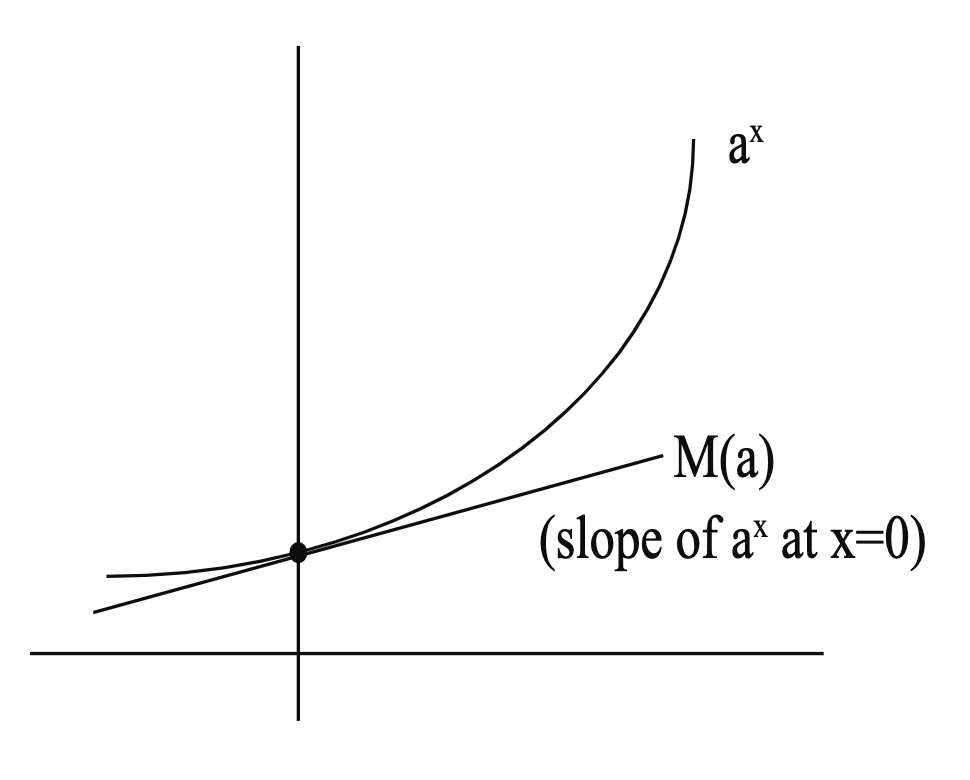
\includegraphics[scale=0.4]{./images/lecture_6_figure_1.png}
		\caption{Geometric Definition of $M(a)$}
	\end{figure}
\end{enumerate}

The trick to finding out what $M(a)$ is is to beg the question and \underline{define} $e$ as the number such that $M(e) = 1$.
Now can we be sure that there is such a number $e$?
First notice that as the base $a$ increases, the graph gets steeper continuosly and $M(1) = 0$ as $1^x = 1$ which is a constant.
So it must pass a point where $M(a) = 1$.

Thus, we \textit{define} $e$ to be the unique number such that $$ M(e) = 1 $$
or, to put it another way, $$ \lim_{h \to 0} \frac{e^h - 1}{h} = 1 $$
or, to put it still another way, $$\diff{}{x} (e^x) = 1 \text{ at } x = 0 $$
So finally, $$\boxed{\diff{}{x}(e^x) = e^x}$$


\subsubsection{Natural log (inverse of $e^x$)}

$$
\boxed{\text{If } y = e^x, \text{ then } \ln(y) = x} 
$$

Note that $e^x$ is always positive even if $x$ is negative.

Let us use implicit differentiation to find $\diff{}{x} \ln(x)$. Let $w = \ln(x)$. We want to find $\diff{w}{x}$.
\begin{equation*}
\begin{split}
	e^w & = x \\
	\diff{}{x} e^w & = \diff{x}{x} \\
	e^w \diff{w}{x} & = 1 \\
	\diff{w}{x} & = \frac{1}{e^w} = \frac{1}{x} \\
\end{split}
\end{equation*}

$$
\boxed{\diff{}{x} \ln(x) = \frac{1}{x}} 
$$

\subsection*{Finally, what about $\diff{}{x}(a^x)$?} 

\subsubsection{Method 1 : Write base $e$ and use chain rule}

Rewrite $a$ as $e^{\ln(a)}$. 
Then, $ a^x = e^{x \ln(a)} $.
Remember $\ln(a)$ is just a constant not a variable.
$$ \diff{}{x} e^{kx} = ke^{kx} $$
$$ \diff{}{} a^x = \diff{}{x} e^{\ln(a)x} = \ln(a)e^{\ln(a)x} = \ln(a)a^x $$
$$ \boxed{\diff{}{x}(a^x) = \ln(a)a^x}$$


\subsubsection{Method 2 : Logarithmic Differentiation}

The idea is to find $\diff{}{x}f(u)$ by finding $\diff{}{x} \ln(f(u))$.

Let, $y = f(u)$ then $\ln(y) = \ln(f(u))$.
Implicitly differentiating to get $\frac{1}{y}\diff{y}{x} = \ln(f(u))'$

Thus, $$\diff{f}{x} = f\ln(f)'$$

Apply this to $f(x) = a^x$.
$$ \ln f(x) = x \ln a \Rightarrow \diff{}{x} \ln f(x) = \ln a $$

Remember $\ln a$ is a constant. Hence, 
$$ \diff{}{x} \ln f(x) = \frac{1}{f(x)} \diff{}{x} f(x) = \ln (a) \Rightarrow f'(x) = \ln(a)f(x) \Rightarrow f'(x) = \ln(a)a^x $$


\subsubsection{Example 1. $\diff{}{x}(x^x) = ?$}

\begin{equation*}
\begin{split}
	f & = x^x \\
	\ln f & = x \ln x \\
	(\ln f)' & = 1 \cdot \ln x + x \cdot \frac{1}{x} \\
	\frac{f'}{f} & = (\ln x + 1) \\
	f' & = x^x(\ln x + 1) \\
\end{split}
\end{equation*}

You can do the same thing by writing $f(x) = e^{x \ln x}$.

\subsubsection{Example 2.}
Evaluate using logs $$ \lim_{k \to \infty} \left( 1+\frac{1}{k} \right)^k $$

Since the exponent changes, its better to find the limit of the logarithm.
$$ 
\lim_{k \to \infty} \ln \left[ \left( 1 + \frac{1}{k} \right)^k \right] 
	= \lim_{k \to \infty} k \ln \left( 1 + \frac{1}{k} \right)
$$

We can substitute $h = 1/k$ so as $k \to \infty, h \to 0$.
$$ \lim_{h \to 0} \frac{\ln(1+h)}{h} $$

Since, $\ln 1 = 0$. We get,
$$ \lim_{h \to 0} \frac{\ln(1+h) - \ln 1}{h} = \diff{}{x} \ln x \big|_{x=1} = 1 $$

Now, the log of the limit is $1$. So the actual limit is $e^1 = e$.
$$ \lim_{k \to \infty} \left( 1 + \frac{1}{k} \right)^k = e $$

This gives us a nice formula to calculate $e$ and with just $k = 10$ gives us a pretty good approximation.


\subsection{Extending Power Rule to Real Numbers}

Earlier we saw that $\diff{}{x} x^n = nx^{n-1}$ is valid for all rational numbers.
Now we will extend it to all real numbers. 

We can write $x^n$ as $e^{n \ln x}$ so that we get
$$ \diff{}{x} x^n = \diff{}{x} e^{n \ln x} 
	= e^{n \ln x} \diff{}{x} (n \ln x)
	= x^n \cdot n \cdot \frac{1}{x}
	= n x^{n-1}
$$

Thus, $$ \boxed{ \diff{}{x} x^n = nx^{n-1} } \quad \forall n \in \mathbb{R} $$
